\documentclass[11pt,a4paper]{article}

% ---------------------------------------------------------------------------
% Kleene: a technical report. Build with `make` (latexmk + pdflatex + bibtex).
% ---------------------------------------------------------------------------

\usepackage[utf8]{inputenc}
\usepackage[T1]{fontenc}
\usepackage{lmodern}
\usepackage{microtype}
\usepackage[margin=1in]{geometry}
\usepackage{amsmath,amssymb}
\usepackage{booktabs}
\usepackage{graphicx}
\usepackage{subcaption}
\usepackage{xcolor}
\usepackage{listings}
\usepackage{tikz}
\usetikzlibrary{arrows.meta,positioning,shapes.geometric,calc}
\usepackage[numbers,sort&compress]{natbib}
\usepackage{url}
\usepackage[hidelinks]{hyperref}
\usepackage{enumitem}
\usepackage{tabularx}
\usepackage{array}
\newcolumntype{Y}{>{\raggedright\arraybackslash}X}

\graphicspath{{figures/}}

\definecolor{kwcolor}{RGB}{30,90,160}
\definecolor{cmcolor}{RGB}{110,110,110}
\lstdefinelanguage{CallSQL}{
  morekeywords={SELECT,FROM,WHERE,AND,OR,NOT,EXISTS,CREATE,TABLE,AS,FUNCTION,
    RETURNS,PROMPT,MODEL,BATCH,IMMUTABLE,STABLE,VOLATILE,PROXY,THRESHOLDS,
    WITH,RECURSIVE,UNION,ALL,ORDER,BY,LIMIT,GROUP,CROSS,JOIN,LATERAL,FINAL,
    CALL,EXPLAIN,SET,AGENT,TOOLS,BUDGET,EFFORT,BOOLEAN,TEXT,DOUBLE,JSON,
    DESC,SUM,COUNT,IN,ON,INSERT,INTO,VALUES,HAVING,DISTINCT,CASE,WHEN,THEN,END},
  sensitive=false,
  morecomment=[l]{--},
  morestring=[b]'
}
\lstset{
  language=CallSQL,
  basicstyle=\small\ttfamily,
  keywordstyle=\color{kwcolor}\bfseries,
  commentstyle=\color{cmcolor}\itshape,
  stringstyle=\color{black},
  showstringspaces=false,
  columns=fullflexible,
  keepspaces=true,
  frame=single,
  framerule=0.3pt,
  xleftmargin=4pt,
  xrightmargin=4pt,
  aboveskip=6pt,
  belowskip=6pt,
  breaklines=true
}

\newcommand{\kleene}{\textsc{Kleene}}
\newcommand{\callsql}{CallSQL}
\newcommand{\code}[1]{\texttt{#1}}
\newcommand{\lmap}{\lambda_f}
\newcommand{\lexp}{\kappa_g}
\newcommand{\lrec}{\rho_d}

\title{\textbf{\kleene: Relational Algebra for Recursive Language-Model Calls}\\[4pt]
\large A planner, a budget and a replay-gated playbook for agents that write SQL}
\author{Marcus Elwin\\[2pt]
\normalsize \href{https://github.com/MarcusElwin/kleene}{github.com/MarcusElwin/kleene}}
\date{October 2026 \\[2pt] \small Technical report, version 1 (draft)}

\begin{document}
\maketitle

\begin{abstract}
Recursive Language Models (RLMs) let a model treat its context as a variable in a
REPL and call itself on slices of it. Every published harness gives the model
Python for that REPL. We argue that for this job SQL is the better language, and
we present \kleene, a Rust harness in which the model's only action is to write
\callsql: a PostgreSQL-flavoured dialect in which model calls are scalar and table
functions, tools are table functions or \code{CALL} statements, delegation is a
lateral table call that opens a child session, search is a recursive CTE with a
beam limit, and the answer is a relation. Because the work is a query, three
things follow that a tool-calling loop cannot offer. A \emph{planner} sees the
cost of every call predicate and applies eight rewrite rules (cheap-first,
memo dedupe, batching, proxy cascades, semi-joins for \code{EXISTS}, beam-limited
recursion, join ordering with branch-and-bound, volatility fences) with a cost
model that \code{EXPLAIN} shows before any money is spent. \emph{Budgets} in
calls, tokens, dollars, depth and wall clock are query semantics: a statement
whose estimate exceeds what remains is refused with its plan. \emph{Learning} is
rows in DuckDB: solved SQL becomes a playbook only after a replay evaluation
with the memo bypassed wins on solves and cost, and every adoption is tied to the
evaluation that admitted it. We describe the algebra, the system and a benchmark
harness with seven task packs run under three modes (learning, frozen, and a
plain tool-calling agent on the same provider and budgets). On the first four
packs Claude Opus~5.5 solves every task in every mode, so they separate on cost
only: the playbook cuts calls per task by 16--39\%, the replay gate costs more
than the playbook saves at twenty tasks a pack, and the one-call baseline is
cheapest wherever the context fits in a prompt. On three harder packs, Claude
Haiku~4.5 separates on accuracy: on rubric-graded memos learning beats frozen
11/20 to 8/20 at a fifth of the calls, while on code-editing episodes both
\kleene{} modes solve 2/12 and the plain agent none. We report these numbers
with their confounds (shared memo between modes, a stopped sweep, one run per
cell) and the fixes they forced.
\end{abstract}

\section{Introduction}
\label{sec:intro}

Recursive Language Models~\citep{zhang2025rlm} change what an agent harness
hands the model. Instead of a prompt that holds the whole context, the root model
sees only the task; the context lives as a variable in a REPL, and the model
writes code that peeks at it, partitions it, and calls \code{llm\_query} or
\code{rlm\_query} on slices. The strategies that emerge (peek, grep,
partition-and-map, summarise, solve in code) are what one would write by hand,
and the paper reports large gains on long-context aggregation at cost parity.
The official harness and every reimplementation we know of give the model
Python for that REPL. A reproduction study~\citep{wang2026reproducing} found that
recursion beyond depth one already degrades on current models, through format
collapse and runaway sub-calls: the freedom of a general-purpose language is
also the freedom to spend without a plan.

\kleene{} starts from a different premise. The REPL is a relational engine and the
model writes SQL. Three properties of SQL make it a better fit for exactly this
job.

\begin{enumerate}[leftmargin=1.5em,itemsep=2pt]
\item \textbf{It is declarative.} The model says \emph{what} relation it wants.
  The harness decides how many calls to make, in what order, concurrently or not,
  and on which model. That is precisely the freedom a planner needs and that an
  imperative loop denies it.
\item \textbf{It has an algebra with known complexity.} Select-project-join is
  NP-complete in combined complexity~\citep{chandra1977conjunctive}, full
  relational algebra is PSPACE-complete~\citep{vardi1982complexity}, and
  \code{WITH RECURSIVE} reaches Datalog and beyond~\citep{dantsin2001complexity},
  up to Turing completeness with \code{UNION ALL}~\citep{gierth2010cyclic}. Every
  statement the model writes can be labelled with the fragment it lives in, and
  join ordering over call predicates is a combinatorial search the planner
  deliberately confronts~\citep{ibaraki1984optimal}.
\item \textbf{The trace is a relation.} Calls, tokens, dollars and depths land in
  DuckDB tables~\citep{raasveldt2019duckdb}. The model, the harness and the
  person inspect execution with the language they drive it with.
\end{enumerate}

Once the work is a query, a planner, budgets and learning fall out as database
problems rather than prompt engineering. This report describes the resulting
system and what it has measured so far. Our contributions are:

\begin{itemize}[leftmargin=1.5em,itemsep=2pt]
\item \callsql{}, a dialect in which model calls, tools, delegation and budgets
  are first-class (\S\ref{sec:callsql}), and a \emph{call algebra} that
  attaches a call kind and a cost signature to any relational operator that
  evaluates a call (\S\ref{sec:algebra}).
\item A planner with eight rewrite rules and a cost model that mirrors the
  executor's short-circuit semantics, exposed through \code{EXPLAIN} and used
  to refuse statements a budget cannot pay for (\S\ref{sec:planner}).
\item A session loop with memoised calls, concurrent child sessions and a
  persistent store in which every learned object (playbook SQL, ratings,
  generator dials, refined prompt functions) is a versioned table adopted
  only after a replay evaluation (\S\ref{sec:system}, \S\ref{sec:learning}).
\item A benchmark harness with seven task packs, three modes that isolate the
  playbook and the SQL abstraction respectively, code and rubric oracles,
  and record-and-replay (\S\ref{sec:bench}); and the results of two real-model
  runs, reported with their confounds (\S\ref{sec:results}).
\end{itemize}

What this report does \emph{not} claim is a benchmark win. The first four packs
were sized for a weaker model and saturate under Opus~5.5; the harder packs
separate on accuracy but have been run once, partially, on Haiku~4.5. The
numbers say where the abstraction pays for itself and where it does not, and
\S\ref{sec:limits} lists what remains before a stronger claim can be made.

\section{\callsql: the language the model writes}
\label{sec:callsql}

Everything the model does in a session is one or more \callsql{} statements in a
single \code{sql} fence. The relational core is a PostgreSQL-flavoured subset:
\code{SELECT} with CTEs and \code{WITH RECURSIVE}, inner and lateral joins,
\code{EXISTS}, \code{IN}, scalar subqueries, grouping, ordering, set operations,
\code{VALUES}, \code{CREATE TABLE \ldots{} AS}, \code{INSERT} and \code{DROP}, over
the types \code{BOOLEAN}, \code{BIGINT}, \code{DOUBLE}, \code{TEXT}, \code{JSON}
and \code{VECTOR}. Three-valued logic short-circuits \code{AND} and \code{OR}
left to right, which the planner relies on. The core is tested differentially
against DuckDB, recursive CTEs included (\S\ref{sec:deterministic}). On top of
it sit five additions.

\paragraph{Context as a table.} A run that is given a context starts with
\code{ctx(ordinal, text)}, one row per paragraph. The root model sees the task,
the catalog and the row count, not the text. It peeks with \code{SELECT \ldots{}
LIMIT}, filters with \code{grep} or \code{LIKE}, partitions with \code{chunks},
and never has to hold the context in its prompt.

\paragraph{Model calls as functions.} The scalar builtins \code{llm(prompt)}
(with optional alias and effort arguments), \code{llm\_bool(prompt)} and
\code{llm\_json(prompt, schema)} each cost one call per distinct argument tuple. \code{expand(text, n)} is a table
builtin that returns $n$ successors. Prompt-defined functions give a call a name,
a return type, a model tier and a volatility:

\begin{lstlisting}
CREATE FUNCTION mentions_hours(note TEXT) RETURNS BOOLEAN
  AS PROMPT 'Does this note record hours worked? {note}'
  MODEL 'proxy' BATCH 20 IMMUTABLE;

CREATE FUNCTION is_valid(c TEXT) RETURNS BOOLEAN
  AS PROMPT 'Is {c} a valid answer to the task?'
  MODEL 'worker' PROXY plausibility THRESHOLDS (0.2, 0.8);
\end{lstlisting}

\code{MODEL} picks a routing alias (\code{root}, \code{worker}, \code{proxy},
\code{judge}, or any alias the router knows). \code{BATCH n} marks a prompt
batchable: the executor answers up to $n$ distinct tuples per call, and the
planner prices $\lceil \text{rows}/n \rceil$ calls. \code{PROXY} declares a cheap
scorer the planner may cascade the predicate through. Bodies may also be SQL
(\code{AS SQL (SELECT \ldots)}) or a shell command (\code{AS SHELL}); volatility
defaults to \code{IMMUTABLE} for prompts, \code{STABLE} for SQL and
\code{VOLATILE} for shell.

\paragraph{Tools.} Pure tools are table functions usable in \code{FROM}:
\code{files}, \code{lines}, \code{read}, \code{grep}, \code{chunks}, \code{env},
\code{git\_log}, \code{git\_diff}, \code{git\_blame}. Side effects run as
statements: \code{CALL shell(cmd)}, \code{CALL write\_file(path, text)},
\code{CALL patch(path, old, new)}, \code{CALL web\_search(q)}, and so on. A
tool's output relation is rendered back to the model like any other result.
Roles restrict which tools a session may use.

\paragraph{Delegation.} \code{rlm(question [, context])} in a \code{CROSS JOIN
LATERAL} opens one child session per input row at depth $d+1$ and returns
\code{(answer, detail)}. \code{CREATE AGENT} declares a role with a model, an
effort, a tool list, a budget and a prompt; \code{spawn('role', task)} runs it.
A child's catalog is restricted to its role's tools and its budget is the
parent's remaining slice intersected with the role's budget.

\begin{lstlisting}
CREATE TABLE parts AS
  SELECT (ordinal / 20) AS part, string_agg(text, '\n') AS chunk
  FROM ctx GROUP BY 1;

CREATE TABLE answers AS
  SELECT p.part, r.answer
  FROM parts p CROSS JOIN LATERAL rlm(
    'Total hours per project in these notes, as project: hours', p.chunk) r;
\end{lstlisting}

\paragraph{Finishing, budgets and plans.} \code{FINAL FROM (query)} ends the
session with that relation as the answer. \code{SET} adjusts effort, model, memo
and the budget dimensions within a session. \code{EXPLAIN} prints the call plan
(\S\ref{sec:planner}); \code{EXPLAIN ANALYZE} runs it and prints actuals beside
estimates. The harness runs the planner on every statement before execution,
and a statement whose estimate exceeds the remaining budget is returned to the
model as a refusal carrying the plan rather than executed.

The opening example of the repository shows the shape the design is built for:

\begin{lstlisting}
SELECT candidate
FROM possibilities
WHERE VERIFY(candidate)
  AND NOT EXISTS (
    SELECT 1 FROM counterexamples ce
    WHERE REFUTE(candidate, ce.text));
\end{lstlisting}

\code{VERIFY} is one call per distinct candidate. The \code{NOT EXISTS} is an
anti-semi-join that stops on the first refuting counterexample: the
counterexample-guided loop of CEGIS and CEGAR~\citep{solarlezama2006combinatorial,
clarke2000cegar} written relationally. \code{EXPLAIN} says how many calls that
is before they are made.

\section{The call algebra}
\label{sec:algebra}

The ordinary operators are selection $\sigma$, projection $\pi$, join
$\bowtie$, union $\cup$, difference, aggregation $\gamma$ and the least fixpoint
$\mu$ for recursive CTEs. \kleene{} adds a \emph{call kind} to any operator that
evaluates a call expression (Table~\ref{tab:callkinds}). The cost of an operator
is the number of calls it implies times the per-alias token and dollar factors
of the function it calls; selectivity of a boolean call predicate is a prior
until the predicate has been observed, after which the sampled pass rate is
used.

\begin{table}[t]
\centering
\small
\begin{tabularx}{\textwidth}{@{}l Y l@{}}
\toprule
Operator & Meaning & Cost signature \\
\midrule
$\lmap$ (map-call) & scalar call $f$ per distinct input tuple & $|\delta(R)| \times \text{tokens}(f)$ \\
$\lexp$ (expand-call) & table call $g$ per input tuple (\code{LATERAL g(\ldots)}) & $|R| \times \text{tokens}(g)$; output = branching factor \\
$\lrec$ (recurse) & \code{rlm} / \code{spawn} at depth $d$ & the child's whole plan \\
$\sigma_{\text{llm}}$, $\bowtie_{\text{llm}}$ & filter or join whose predicate contains a call & inherits $\lmap$; $|R \times S|$ calls for a join unless rewritten \\
\bottomrule
\end{tabularx}
\caption{Call kinds. $\delta$ is duplicate elimination; identical prompts cost one call.}
\label{tab:callkinds}
\end{table}

Every statement is also labelled with the fragment it lives in: CQ for
select-project-join, FO for the full relational algebra, REC when a recursive
term is present. The badge is a reminder that a recursive call plan is a
program, not a lookup.

\subsection{Rewrite rules and the cost model}
\label{sec:planner}

The planner in \code{kleene-algebra} runs rules over the annotated plan until
nothing changes. All eight are standard query-rewrite shapes applied to call
costs.

\begin{enumerate}[leftmargin=1.5em,itemsep=1pt]
\item \textbf{Cheap first.} $\sigma_{\text{pure}} \circ \sigma_{\text{llm}}
  \equiv \sigma_{\text{llm}} \circ \sigma_{\text{pure}}$: pure conjuncts run
  before call conjuncts, in filters and in join conditions. Because estimates
  mirror the executor's left-to-right short-circuit, the saving is visible in
  the numbers rather than assumed.
\item \textbf{Dedupe then map.} $\lmap(R) \equiv \lmap(\delta(R)) \bowtie R$,
  backed by a persistent memo keyed on model and prompt fingerprint and shared
  across sessions and runs.
\item \textbf{Batch.} $\lmap$ over $n$ tuples of a \code{BATCH n} function becomes
  one call with $n$ items, priced $\lceil \text{rows}/n \rceil$. An answer that
  does not hold exactly one element per item falls back to one call per tuple.
\item \textbf{Cascade.} $\sigma_{\text{oracle}}(R)$ with a declared proxy becomes
  $\text{score} \ge \tau_{\text{hi}} \;\vee\; (\text{score} \ge \tau_{\text{lo}}
  \wedge \text{oracle})$, applied when the priced cascade is cheaper; the shape
  is LOTUS's~\citep{patel2025semantic}, with thresholds declared rather than
  calibrated (\S\ref{sec:limits}).
\item \textbf{Semi-join.} \code{[NOT] EXISTS} with a call predicate becomes a
  semi or anti join that stops at the first (counter)example instead of
  materialising the cross product.
\item \textbf{Beam-limited recursion.} Inside $\mu$, a trailing \code{ORDER BY
  \ldots{} LIMIT k} in the recursive term keeps the best $k$ new rows of each
  round: breadth-first search with a model successor function becomes beam
  search of width $k$, and the planner simulates the fixpoint round by round
  to price it.
\item \textbf{Join ordering.} Dynamic programming over relation subsets with
  branch-and-bound, in the tradition of~\citet{selinger1979access} and
  \citet{moerkotte2006analysis}: each split is priced with the predicates that
  first become applicable there, pure conjuncts narrowing the pairs and call
  conjuncts paying one call per surviving pair.
\item \textbf{Volatility fences.} Rules 1--7 move operators only across
  \code{IMMUTABLE} and \code{STABLE} operators. A \code{VOLATILE} operator (a
  shell command, a file write) is a fence: nothing crosses it, it is never
  deduplicated, and its input order is preserved. The planner trusts the label,
  so a side effect is never marked anything else.
\end{enumerate}

Estimates use the store's row counts, sampled selectivities, per-alias cost
factors and pricing. \code{EXPLAIN} prints the plan as a tree with per-node
rows, calls, tokens and dollars, the call kinds, the fences, the fragment
badge, the rules that fired, the join-order plan space and the alternatives it
priced.

\paragraph{Budgets as semantics.} A \code{Budget} has calls, tokens, dollars,
depth and wall clock. A child session receives the parent's remaining slice
intersected with its role's budget, and its spending rolls up. Exceeding a
budget cancels the statement, not the session, and returns a budget row to the
model; a statement whose \emph{estimate} already exceeds the remainder is
refused before it runs. Depth defaults to a cap of two, following the
reproduction study's finding that deeper recursion degrades on current
models~\citep{wang2026reproducing}; it is a dial, not a constant.

\section{System}
\label{sec:system}

\kleene{} is a Rust workspace of eleven crates with a shared interface crate
(\code{kleene-core}: values, schemas, the catalog, budgets, call kinds) that
every other crate depends on. Figure~\ref{fig:turn} shows the path of one turn.

\begin{figure}[t]
\centering
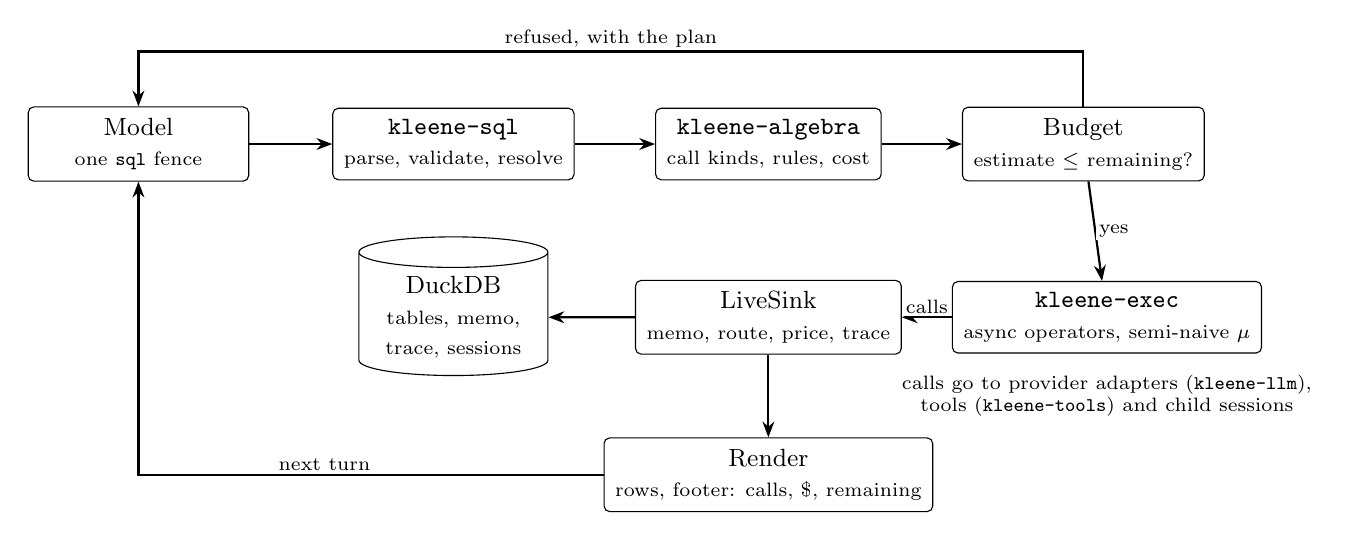
\begin{tikzpicture}[
  box/.style={draw, rounded corners=2pt, align=center, font=\small,
              minimum height=9mm, minimum width=28mm, inner sep=4pt},
  store/.style={draw, cylinder, shape border rotate=90, aspect=0.2,
                align=center, font=\small, minimum height=12mm, minimum width=24mm, inner sep=3pt},
  arr/.style={-{Stealth[length=2mm]}, thick},
  lbl/.style={font=\scriptsize, fill=white, inner sep=1pt}
]
\node[box] (model) at (0,0) {Model\\{\scriptsize one \code{sql} fence}};
\node[box] (sql) at (4,0) {\code{kleene-sql}\\{\scriptsize parse, validate, resolve}};
\node[box] (alg) at (8,0) {\code{kleene-algebra}\\{\scriptsize call kinds, rules, cost}};
\node[box] (budget) at (12,0) {Budget\\{\scriptsize estimate $\le$ remaining?}};
\node[box] (exec) at (12.3,-2.2) {\code{kleene-exec}\\{\scriptsize async operators, semi-naive $\mu$}};
\node[box] (sink) at (8,-2.2) {LiveSink\\{\scriptsize memo, route, price, trace}};
\node[store] (db) at (4,-2.2) {DuckDB\\{\scriptsize tables, memo,}\\{\scriptsize trace, sessions}};
\node[box] (render) at (8,-4.2) {Render\\{\scriptsize rows, footer: calls, \$, remaining}};
\node[font=\scriptsize, align=center, below=1.5mm of exec] (ext) {calls go to provider adapters (\code{kleene-llm}),\\tools (\code{kleene-tools}) and child sessions};

\draw[arr] (model) -- (sql);
\draw[arr] (sql) -- (alg);
\draw[arr] (alg) -- (budget);
\draw[arr] (budget) -- node[lbl, right] {yes} (exec);
\draw[arr] (exec) -- node[lbl, above] {calls} (sink);
\draw[arr] (sink) -- (db);
\draw[arr] (sink) -- (render);
\draw[arr] (render.west) -| node[lbl, pos=0.3, above] {next turn} (model.south);
\draw[arr] (budget.north) |- ++(0,7mm) -| node[lbl, pos=0.25, above] {refused, with the plan} (model.north);
\end{tikzpicture}
\caption{One turn of a session. The harness sends a cached system prefix (rules,
catalog, budget) plus the transcript; the model replies with \callsql; the
statement is parsed, annotated, priced, checked against the budget, executed
through a sink that memoises, routes and traces every call, and rendered back.
The loop repeats until \code{FINAL}.}
\label{fig:turn}
\end{figure}

\paragraph{Execution.} Operators are pull-based async streams of small columnar
batches. Recursion runs by semi-naive evaluation~\citep{bancilhon1986amateur}:
each round joins only the previous round's delta against the recursive term, so
calls in that term run only on new rows, and a round is one awaitable unit the
UI can show as a frontier size. Model calls are concurrent under a per-session
semaphore with a provider rate limiter; ordered results are preserved.

\paragraph{The sink.} Every scalar, table, tool or child call passes through a
\code{LiveSink} that looks the call up in the memo, and on a miss routes it to a
provider alias, prices it at the router's list rates, charges the budget, stores
the response in the memo and emits a trace event. Identical prompts are
therefore free the second time, across sessions and runs; this is also how a
recorded run replays offline.

\paragraph{Sessions and delegation.} Child sessions are the same loop one level
deeper with a role, a budget slice and their own table namespace; a child's
\code{FINAL} returns to the parent as a row. Children of one lateral call run
concurrently. Session state (tables, transcript, budget) lives in the store, so
killing the process and running \code{kleene resume} continues where it stopped;
checkpointing is a property of the storage, not a feature.

\paragraph{Model layer.} Adapters speak the Anthropic Messages and
OpenAI-compatible wire formats directly over HTTPS, plus an Open Responses
adapter behind a feature flag; there are no vendor SDKs. A router maps aliases
to models and prices, and a \code{ReplayProvider} serves recorded fixtures so
the test suite and the benchmark harness can run without a key. Two provider
facts the benchmarks forced into the adapter are described in
\S\ref{sec:haiku}.

\paragraph{Store and trace.} DuckDB holds session tables, the memo, the trace
(\code{trace\_sessions}, \code{trace\_statements}, call events), the continual
loop's tables and the benchmark rows. \code{kleene trace} runs plain DuckDB SQL
over all of it, and the terminal UI's \code{/trace} does the same from the
prompt.

\paragraph{Processes.} \code{kleene run}, \code{repl}, \code{explain},
\code{learn} and \code{bench} run the harness in one process. The terminal UI
talks to an engine daemon over a Unix socket with a JSONL protocol with cursors,
so a reconnecting client resumes from where it left off and \code{kleene attach}
watches the same events headless. The UI is one scrolling stream: the model's
reply streams in, each fence runs as it lands, every statement shows its rows
and its cost, child sessions nest under the turn that opened them.

\section{Learning as tables}
\label{sec:learning}

The continual loop (\code{kleene learn}) is itself a query over a \code{tasks}
table: pick the next pending task by curriculum policy, run a session, judge
\code{FINAL} with the task's oracle, record outcome and cost, repeat. Two things
keep it alive: generators that keep the table non-empty, and learning that
changes how the next task is attempted.

\paragraph{Tasks and difficulty.} Generators (\code{sat3}, \code{graph},
\code{puzzle}, \code{corpus}, \code{repo}, \code{statements},
\code{contracts}, \code{logbook}, \code{memo}) produce tasks deterministically
from a hardness dial in $[0,1]$ and a seed, each with a code oracle; the design
follows Reasoning Gym~\citep{stojanovski2025reasoninggym} and the random 3-SAT
phase transition~\citep{mitchell1992hard}. Every task and every solver
configuration carries a rating moved by a Bradley--Terry
model~\citep{bradley1952rank} over solve and fail outcomes: a task that beats
strong configurations is hard, a configuration that beats hard tasks is strong.
The curriculum samples the pending task nearest even odds for the current
solver, steps a generator's dial up when its solve rate exceeds 0.7 and down
below 0.3, in the spirit of the learnability target of Absolute Zero
Reasoner~\citep{zhao2025absolutezero}.

\paragraph{What is learned.} Nothing here updates weights. Each learned object
is a table with a version and a provenance pointer:

\begin{itemize}[leftmargin=1.5em,itemsep=1pt]
\item the \textbf{playbook}: SQL that solved a task, keyed by task kind,
  rendered into the cached prefix as examples for similar tasks and queryable
  by the model;
\item \textbf{refined prompt functions} (\code{learn refine}): new versions of
  \code{VERIFY}-style functions in a ledger with before/after snapshots and
  rollback;
\item the \textbf{cost model}: sampled selectivities of boolean call predicates
  that feed the planner (today per session; \S\ref{sec:limits});
\item \textbf{ratings} of tasks and solver configurations, and each generator's
  \textbf{dial}.
\end{itemize}

\paragraph{The replay gate.} A candidate playbook entry is adopted only after a
replay evaluation: the harness re-runs a sample of earlier tasks of the same
kind in two arms, with and without the candidate, with the memo bypassed, and
adopts the entry only if the arm with it wins on solves and costs no more. The
sample is three tasks by default, so a gate costs six task runs per solved
task. Every adoption is tied in \code{playbook\_evals} to the evaluation that
admitted it, and \code{learn playbook} lists reverts, so a regression can be
traced to the entry that caused it. The base system prompt is immutable and
learned content is appended in marked sections. \S\ref{sec:opus} shows that at
twenty tasks a pack the gate spends far more than the playbook saves; it is the
price of never adopting an entry on faith.

\section{Benchmark methodology}
\label{sec:bench}

The harness's claim is specific: a model writing \callsql{} over a relational
engine solves the same tasks as a tool-calling agent for fewer calls and
dollars, and the harness gets better over a stream of tasks because solved SQL
is kept. The benchmark harness (\code{kleene bench}) is built to test exactly
that, so every run records three things per task: was it solved, how many model
calls it took, and what it cost.

\subsection{Packs}

A pack is a directory with a \code{pack.json}: tasks with text, optional context,
setup commands, a workspace source, an oracle and a difficulty prior.
Table~\ref{tab:packs} lists the seven shipped packs. The synthetic packs are
frozen output of the loop's generators, so two runs see the same tasks in the
same order and \code{bench build} regenerates them byte for byte; the two
long-context packs are stored lazily as (generator, dial, seed) triples and
regenerated on load. The coding pack is hand-written: four small Python
projects, each a three-step \emph{episode} in which the second and third steps
run in the workspace the previous step left, and a step's setup installs the
reference solution for the previous step when its hidden tests fail, so each
step is measured on its own work. The external datasets these packs imitate
(OOLONG~\citep{bertsch2025oolong}, Terminal-Bench~\citep{merrill2026terminalbench},
FinanceBench~\citep{islam2023financebench}, CUAD~\citep{hendrycks2021cuad},
Harvey LAB~\citep{harvey2026lab}, SWE-bench~\citep{jimenez2024swebench}) are not
redistributed; a Harvey LAB checkout imports through \code{bench import-lab}
with LAB's own evaluator as the scorer of record.

\begin{table}[t]
\centering
\small
\begin{tabularx}{\textwidth}{@{}l r Y l l@{}}
\toprule
Pack & $n$ & What the model gets and must produce & Oracle & Stands in for \\
\midrule
\code{terminal} & 6 & a workspace and a shell instruction; files left behind & \code{shell} & Terminal-Bench \\
\code{oolong-like} & 20 & dated meeting notes as \code{ctx}; hours per project & \code{exact} & OOLONG aggregation \\
\code{finance-synthetic} & 20 & a synthetic income statement; one number & \code{number} & FinanceBench \\
\code{legal-synthetic} & 20 & a synthetic contract; the clause categories present & \code{exact} & CUAD / LAB \\
\code{logbook-hard} & 30 & a 30\,000-token work log with corrections and distractors; one of five aggregate questions & \code{exact} & OOLONG at full size \\
\code{memo-rubric} & 20 & a 40-section agreement with an amendment and a rejected proposal; a short memo & \code{judge} & LAB drafting \\
\code{coding} & 12 & a Python project with visible tests; implement, extend, fix a bug & \code{shell} & SWE-bench episodes \\
\bottomrule
\end{tabularx}
\caption{The seven shipped packs. \code{exact} compares row multisets, \code{number}
the first cell within a tolerance, \code{shell} runs a command (here the grader's
hidden tests) and \code{judge} asks a separate model for \code{PASS} against a
rubric that names every required fact and forbids the superseded values.}
\label{tab:packs}
\end{table}

\subsection{Modes}

Every pack runs under one of three modes, and two comparisons fall out of them.

\begin{description}[leftmargin=1.5em,itemsep=1pt]
\item[\code{learning}] \kleene{}: the model writes \callsql, the playbook is
  shown, candidates are recorded and adopted through the gate, ratings move.
\item[\code{frozen}] \kleene{} with the same model, tools and budgets, but no
  playbook shown, no candidate recorded, no rating moved. The control for
  learning.
\item[\code{plain}] a tool-calling agent on the same provider, tools and
  budgets, in the ReAct shape~\citep{yao2023react}: each turn the model returns
  one JSON action and tool output comes back as text. The baseline for cost
  parity, as in the RLM paper's framing: same model, same spend, only the
  abstraction differs.
\end{description}

\code{learning} against \code{frozen} isolates the playbook; \code{frozen}
against \code{plain} isolates the SQL abstraction. Two caveats matter for
reading the results. Both \kleene{} modes read the same store, so a frozen run
on a store that has seen a learning run (or the reverse) is served from the
memo for every prompt already sent; a clean comparison needs a fresh store per
mode, which the Haiku run did not yet do (\S\ref{sec:haiku}). And the plain
agent parses JSON actions from text rather than using a vendor's native
tool-calling API, which keeps it provider-agnostic but is not identical to a
vendor agent loop.

\subsection{What is recorded}

\code{bench run} writes one row per task to \code{evals}: run, pack, mode,
position in the stream, task, solved, the oracle's reason, calls, tokens,
dollars, deepest child, turns and wall clock. \code{bench report} aggregates by
pack and mode; \code{bench csv} exports the rows; \code{bench curve} prints the
rolling solve rate of one run; \code{bench plot} draws five standalone SVGs
(learning curve, accuracy at cost parity, calls against difficulty, planner
estimate against actual, plan-space size against query shape) without a
plotting library. The replay evaluations a learning run pays for are recorded
in \code{playbook\_evals} with their own dollars and are \emph{not} in
\code{evals}; the true cost of a learning run is the sum. \code{bench run
--record} saves every model reply as a fixture and \code{--replay} serves it
back, so a run reproduces offline; \code{--resume} continues a run that a
provider error stopped.

\section{Results}
\label{sec:results}

\subsection{Deterministic measurements}
\label{sec:deterministic}

Table~\ref{tab:deterministic} is the part of the evidence that needs no model:
the test suite runs it in CI with scripted providers, code oracles and replay
fixtures.

\begin{table}[t]
\centering
\small
\begin{tabularx}{\textwidth}{@{}>{\hsize=0.8\hsize}Y >{\hsize=1.0\hsize}Y >{\hsize=1.2\hsize}Y@{}}
\toprule
Property & Test & Result \\
\midrule
Relational core equals DuckDB & property-based differential suite & passes, recursive CTEs included \\
Join ordering, two call predicates over three relations & estimate and actual calls against a counting sink & as written 12\,000 estimated calls, chosen order 60; actual $\ge 10\times$ fewer with identical rows \\
Plan-space growth & seven-way join & 665\,280 bushy orders priced through 1\,623 subset splits (309 pruned) \\
Cascade & proxy at $0.1\times$ cost, thresholds $(0.2, 0.8)$ & 100 proxy + 60 oracle calls beat 100 oracle calls by estimate; on data the oracle is asked only for the band (5 of 20) \\
Beam recursion & \code{expand} $\times 4$, three rounds & 20 calls with beam 5 against $>100$ unbounded \\
Continual loop & scripted solver over generated puzzles & tasks solved, playbook v1 adopted after a replay eval, ratings and dial move, restart resumes \\
Terminal-Bench-style pack & shell tasks from SQL & tasks solved, oracles run in fresh workspaces \\
Plain-agent baseline & same provider, JSON actions & tool call then final; the control for cost parity \\
\bottomrule
\end{tabularx}
\caption{What the deterministic suite establishes.}
\label{tab:deterministic}
\end{table}

\subsection{Claude Opus 5.5 on the first four packs}
\label{sec:opus}

The four original packs ran once each under the three modes on 27 September
2026 with the default routing: \code{root} on \code{claude-opus-5-5} at high
effort, \code{worker} and \code{judge} on \code{claude-sonnet-5}, \code{proxy}
on \code{claude-haiku-4-5}, priced at the router's list rates.
Table~\ref{tab:opus} gives the per-pack rows; Figure~\ref{fig:opus} the plots
\code{bench plot} drew from the same store. \code{dollars} is the pack total,
calls and tokens are per task, and the learning column excludes the gate.

\begin{table}[t]
\centering
\small
\begin{tabular}{@{}llrrrr@{}}
\toprule
Pack & Mode & Solved & Calls / task & Tokens / task & Dollars \\
\midrule
terminal (6)           & frozen   & 6/6   & 2.17  & 10\,551 & 0.07 \\
                       & learning & 6/6   & 1.33  & 6\,742  & 0.04 \\
                       & plain    & 6/6   & 2.50  & 2\,395  & 0.03 \\
\addlinespace
oolong-like (20)       & frozen   & 20/20 & 4.90  & 30\,778 & 1.51 \\
                       & learning & 20/20 & 3.85  & 41\,991 & 1.92 \\
                       & plain    & 20/20 & 1.00  & 3\,084  & 0.39 \\
\addlinespace
finance-synthetic (20) & frozen   & 20/20 & 3.45  & 42\,177 & 0.83 \\
                       & learning & 20/20 & 2.40  & 29\,999 & 0.63 \\
                       & plain    & 20/20 & 1.00  & 1\,244  & 0.07 \\
\addlinespace
legal-synthetic (20)   & frozen   & 20/20 & 12.65 & 62\,452 & 1.69 \\
                       & learning & 20/20 & 10.60 & 58\,315 & 2.61 \\
                       & plain    & 20/20 & 1.00  & 1\,475  & 0.11 \\
\bottomrule
\end{tabular}
\caption{Claude Opus 5.5, 27 September 2026, one run per cell. Gate replays
(not included): \$1.25 terminal, \$10.70 oolong, \$5.46 finance, \$16.63 legal.}
\label{tab:opus}
\end{table}

\begin{figure}[t]
\centering
\begin{subfigure}[t]{0.78\textwidth}
  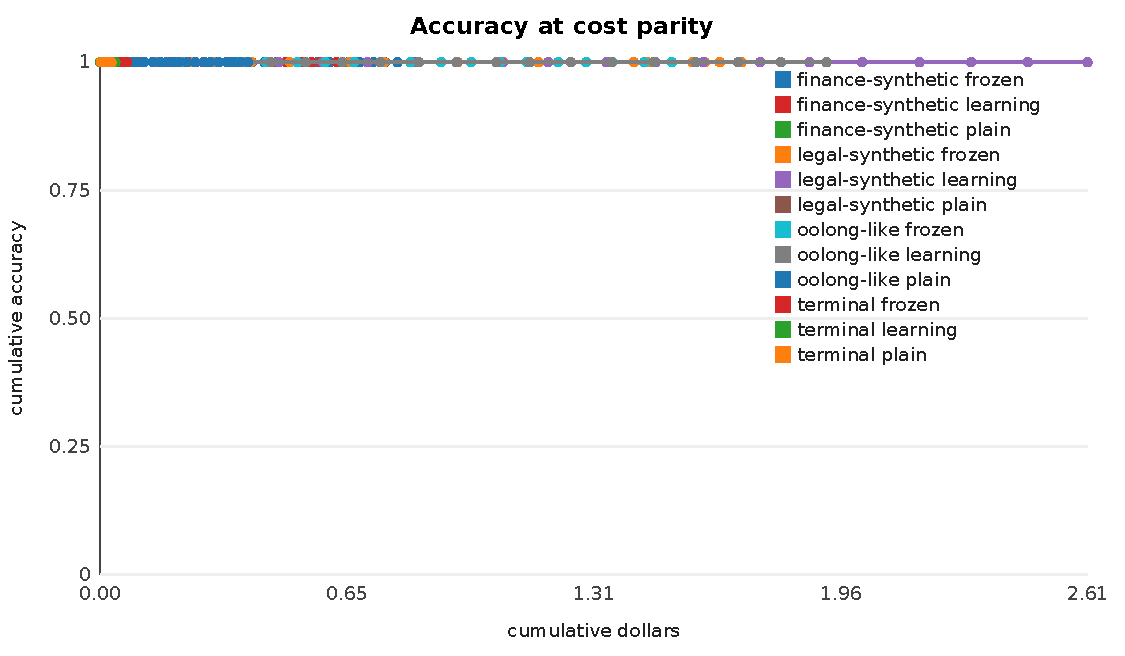
\includegraphics[width=\linewidth]{opus_cost_parity}
  \caption{Cumulative accuracy against cumulative dollars.}
\end{subfigure}\\[6pt]
\begin{subfigure}[t]{0.78\textwidth}
  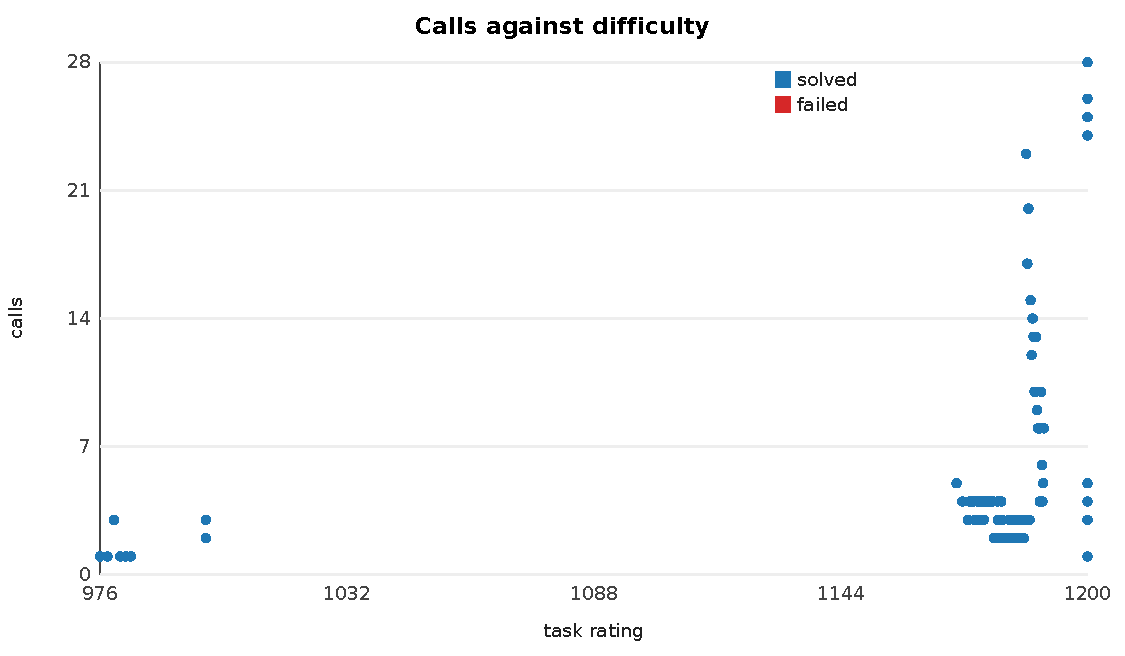
\includegraphics[width=\linewidth]{opus_calls_vs_difficulty}
  \caption{Calls per task against the task's rating.}
\end{subfigure}
\caption{The Opus 5.5 run. Every line reaches accuracy 1; the plot separates the
modes on cost only, with the plain agent leftmost on every pack.}
\label{fig:opus}
\end{figure}

\paragraph{Accuracy is saturated.} Opus 5.5 solves every task of every pack in
every mode. The packs were sized for a weaker model at dial 0.5; they separate
nothing on accuracy, so what follows is about calls and dollars.

\paragraph{The playbook cuts calls per task.} Learning against frozen: terminal
2.17 to 1.33, oolong 4.90 to 3.85, finance 3.45 to 2.40, legal 12.65 to 10.60.
Only two packs adopted anything, though: oolong (16 of 20 candidates) and legal
(5 of 21). On terminal and finance every candidate was rejected because its
replay cost more than the baseline's, so those learning runs are frozen runs
with ratings on, and their call reduction is run-to-run variance, not learning.
On oolong the second half of the learning run took 3.9 calls per task where the
first half took 3.8: most of the gain arrived with the first adopted entries.
On legal the halves are 13.7 and 7.5, the curve the design predicts.

\paragraph{The gate is the cost.} Each candidate is replayed on three earlier
tasks in both arms, six task runs per solved task, and those replays cost
\$1.25, \$10.70, \$5.46 and \$16.63 on the four packs against \$0.04, \$1.92,
\$0.63 and \$2.61 for the counted runs. At twenty tasks a pack the gate spends
far more than the playbook saves. It earns its keep only over a long stream, and
a cheaper gate (a smaller sample, a proxy model, a cached baseline arm) is the
obvious next change.

\paragraph{The plain agent wins on cost here.} Every context in these packs fits
in one prompt (under 4\,000 characters), so the baseline answers in one call
with no tool use: \$0.39 against \$1.51 on oolong, \$0.07 against \$0.83 on
finance, \$0.11 against \$1.69 on legal. The SQL abstraction pays for a catalog,
a planner and a transcript of rendered results on every turn, and at this scale
that is pure overhead. The claim of \S\ref{sec:intro} is about work that does
not fit in one call; these packs do not test it, and the numbers say so.

\paragraph{Per-clause calls are cheap and visible.} On legal the model
classified clause by clause with a prompt function on the \code{worker} alias,
up to 26 calls a task at about \$0.10: the $\lmap$ map-call doing what it is
for, many small calls on a cheap model, priced before they run.

\paragraph{Costs drift up within a run.} Per-task dollars on oolong learning
rose from \$0.084 in the first half to \$0.107 in the second while calls stayed
flat. Two things grow the prompt: the adopted playbook entries, and, as it
turned out, the scratch tables every session created in the shared store, which
the catalog listed to every later session (287 such tables after these runs).
The second was a bug: it also changed the prompt fingerprint from task to task,
so a recorded run could not be replayed from its own fixtures. Bench sessions
now drop their tables when they finish.

\subsection{Claude Haiku 4.5 on the harder packs}
\label{sec:haiku}

The harder packs ran on 1 October 2026 with every solver alias on
\code{claude-haiku-4-5-20251001} and the \code{judge} alias on
\code{claude-sonnet-5-5}. The sweep was stopped before it finished;
Table~\ref{tab:haiku} is what completed. Not in the table: \code{logbook-hard}
in any mode (a frozen task took about 500 calls and over twenty minutes at
Haiku's pace, so the pack was capped at ten tasks and then stopped before the
first row landed), and \code{coding} in plain mode (below). Gate replays cost
\$1.43 on memo-rubric (11 candidates, 3 adopted) and \$1.04 on coding (2
candidates, 1 adopted); the counted runs cost \$3.36 in all.

\begin{table}[t]
\centering
\small
\begin{tabular}{@{}llrrrr@{}}
\toprule
Pack & Mode & Solved & Calls / task & Tokens / task & Dollars \\
\midrule
coding (12)      & frozen   & 2/12  & 4.58  & 48\,375 & 0.87 \\
                 & learning & 2/12  & 2.67  & 29\,910 & 0.47 \\
\addlinespace
memo-rubric (20) & frozen   & 8/20  & 19.95 & 49\,043 & 1.30 \\
                 & learning & 11/20 & 3.80  & 23\,041 & 0.37 \\
                 & plain    & 8/20  & 3.15  & 10\,764 & 0.35 \\
\bottomrule
\end{tabular}
\caption{Claude Haiku 4.5 solvers with a Sonnet 5.5 judge, 1 October 2026, one
run per cell; the sweep was stopped before \code{logbook-hard} and the coding
plain run produced rows. The learning rows share the frozen rows' memo (see
text).}
\label{tab:haiku}
\end{table}

\begin{figure}[t]
\centering
\begin{subfigure}[t]{0.78\textwidth}
  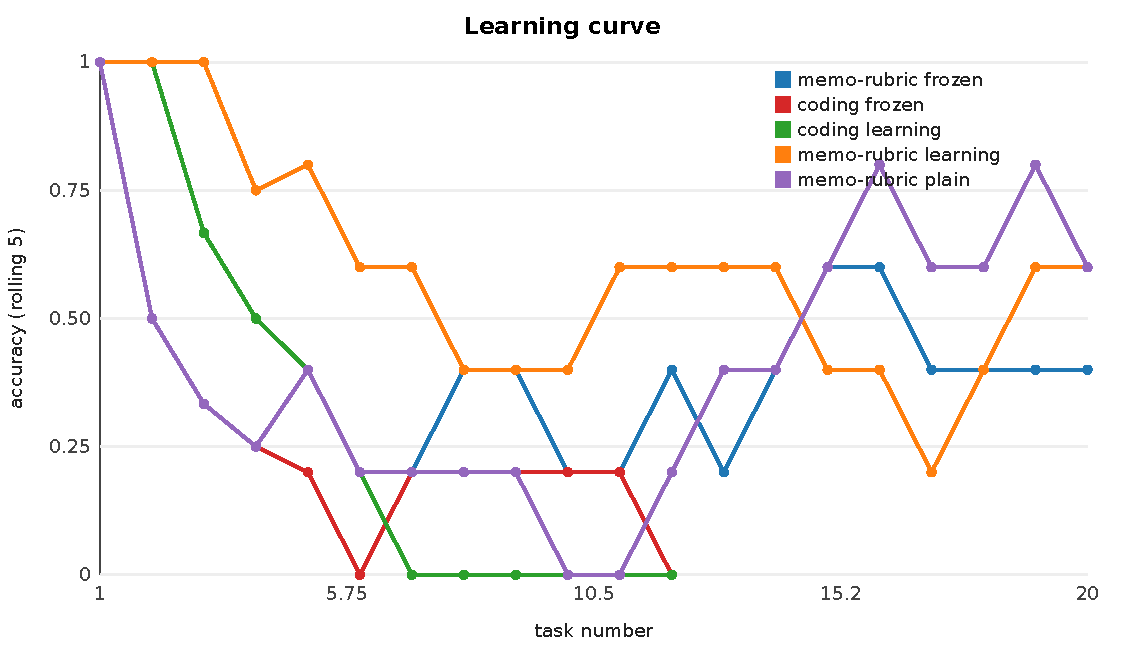
\includegraphics[width=\linewidth]{haiku_learning_curve}
  \caption{Rolling-5 accuracy by position in the stream.}
\end{subfigure}\\[6pt]
\begin{subfigure}[t]{0.78\textwidth}
  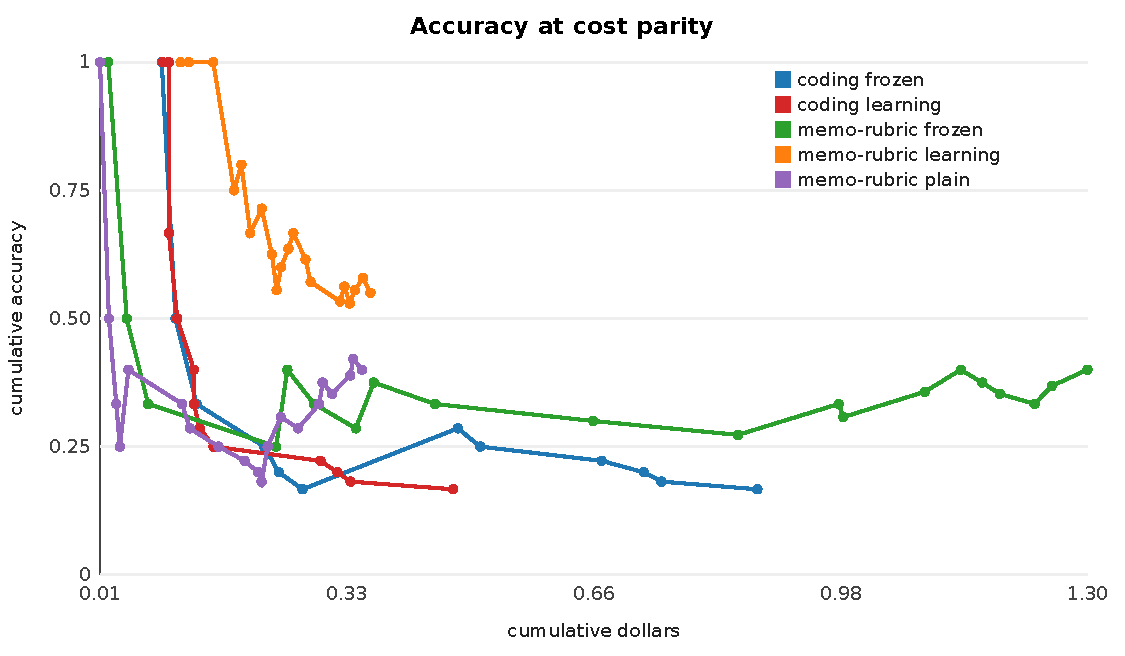
\includegraphics[width=\linewidth]{haiku_cost_parity}
  \caption{Cumulative accuracy against cumulative dollars.}
\end{subfigure}
\caption{The Haiku 4.5 run on \code{memo-rubric} and \code{coding}. On
memo-rubric the learning line ends above frozen and plain at a fraction of
frozen's spend; on coding both \kleene{} lines fall to zero after the first
step of each episode.}
\label{fig:haiku}
\end{figure}

\paragraph{These packs separate on accuracy.} Where Opus 5.5 solved every task
of the first four packs, Haiku solves 17\% of the coding steps and 40 to 55\% of
the memos. The coding steps it solves are the first step of an episode; it
solved no ``extend'' or ``fix the bug report'' step in either \kleene{} mode.

\paragraph{Learning beat frozen on memo-rubric, on both axes.} 11/20 against
8/20, at 3.8 calls a task against 19.95 and \$0.37 against \$1.30. Two effects
are mixed in. Three playbook entries were adopted, and the second half of the
learning run solved 5 of 10 where the frozen run's first half solved 3 of 10.
But most of the frozen run's calls are a failure mode the playbook happens to
steer around: Haiku writes \code{llm\_json} output schemas the API rejects
(\code{additionalProperties} unset, \code{minItems} above 1, a bare
\code{\{"hours": "number"\}}), and the statement retries until the call budget
is gone; five frozen tasks took 22 to 141 calls each. The adapter now rewrites
a model-written schema into the accepted subset before the request; these runs
predate it.

\paragraph{Learning and frozen share the memo.} The learning run came second in
the same store, so a prompt identical to one the frozen run sent was answered
from the memo for free. Two coding steps in the learning run finished with zero
calls: they replayed the frozen run's failed answers. The learning column's
calls and dollars are therefore not an independent measurement; the
documentation now prescribes a fresh store per mode.

\paragraph{The plain baseline needs a protocol the model keeps.} The agent asks
for one JSON action per reply. Haiku answers with five to ten actions and
invented tool output between them; the first extractor took the span from the
first brace to the last, which never parsed, so on every coding task the model
saw only a parse error and gave up after two turns (0/12 at \$0.45). The
extractor now takes the first balanced object and runs it. With that, Haiku
worked through the first coding task for all 30 turns without solving it
(\$1.11) and the rerun was stopped before a row landed. On memo-rubric, where
the task fits in one call, the plain agent matches frozen on accuracy at a
quarter of the cost, and learning beats it by three tasks for the same money.

\paragraph{The judge wobbles.} Sonnet 5.5's first lines included ``PASS (with
caveat)'', ``PASS (provisional)'' and ``PASS or FAIL?'', all counted as passes
by the first parser. It now requires a first line that says PASS and does not
mention FAIL. The memo frozen and learning runs predate that change; the plain
run does not.

\paragraph{Two provider facts.} Haiku rejects the \code{effort} parameter the
adapter sent along with the rest of the model family, so under the default
routing every \code{proxy} call failed until the adapter learned to omit it;
and \code{claude-sonnet-5-5} was served on 1 October where it was not on 27
September.

\subsection{Planner estimates against actuals}
\label{sec:estimates}

The Haiku run was the first made after \code{bench run} began tracing
statements, so its store holds an estimate and an actual call count for each of
the 1\,028 statements the planner priced (Figure~\ref{fig:estimate}). Reading
the plot: 670 statements made no calls and were estimated at none; 254 were
estimated at one call and made one; 82 were estimated at one and made none,
which is the memo answering a repeated prompt. The planner never
under-estimated by more than a call. Where it was wrong it was high, by up to
two orders of magnitude on about a dozen statements, each a per-row call priced
on a table's row count that then failed early or was served from the memo. For
budget refusal that is the safe direction; for the learned cost model it is the
error to drive down.

\begin{figure}[t]
\centering
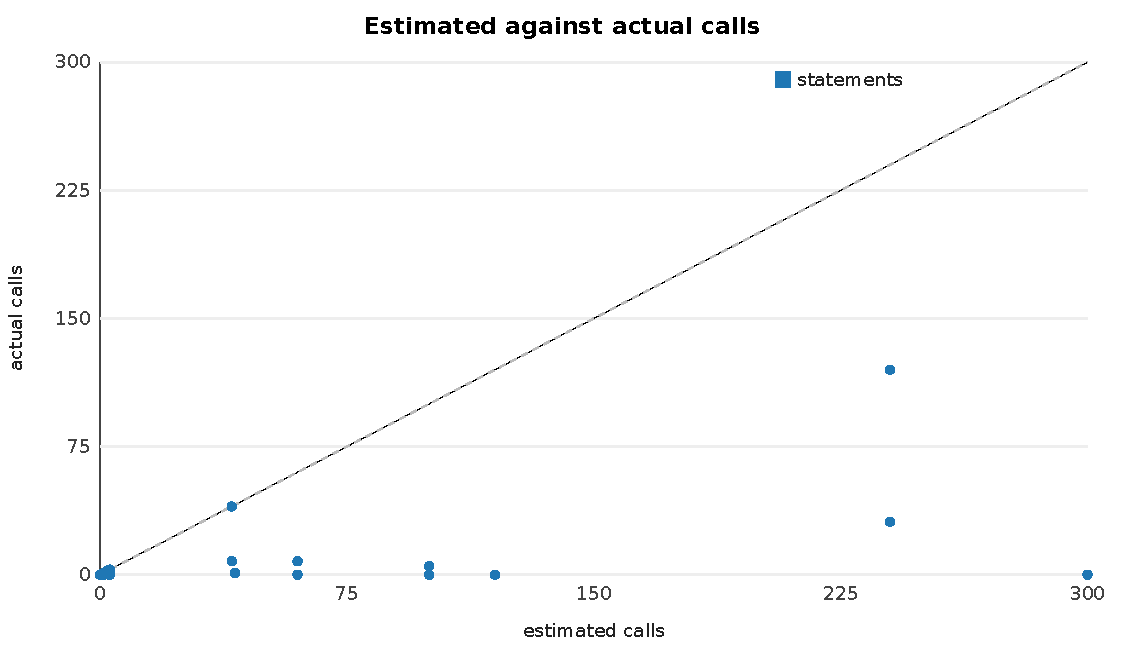
\includegraphics[width=0.6\textwidth]{haiku_estimate_accuracy}
\caption{Estimated against actual calls per statement, Haiku run. Points on the
diagonal are exact; the outliers lie below it (over-estimates).}
\label{fig:estimate}
\end{figure}

\subsection{What the numbers say}

Taken together, the two runs support three statements and refuse a fourth.
First, the planner, the budget and the trace work as designed on real models:
estimates are conservative, refusals carry plans, per-clause calls land on the
cheap alias, and every cost in this section was read from the store. Second,
the playbook does reduce calls per task when something is adopted, and on the
one pack that separates on accuracy it also raised solves, with the confounds
stated. Third, the replay gate, at its current sample size, is the dominant
cost of learning at pack scale. What the runs do not support is the headline
cost-parity claim: wherever the context fits in one prompt the plain agent is
cheaper, and the pack built to test the other case (\code{logbook-hard}, a
30\,000-token context that has to be filtered and aggregated) has not yet
produced a row.

\section{Related work}
\label{sec:related}

\paragraph{Recursive language models.} \citet{zhang2025rlm} introduced the
REPL-variable framing and the \code{llm\_query} / \code{rlm\_query} sub-calls that
\kleene{} maps onto \code{llm} and \code{rlm}; their evaluation suite (OOLONG,
BrowseComp-Plus) is the headline comparison the \code{logbook-hard} pack is
built toward. \citet{wang2026reproducing} reproduced the result and documented
the depth-two degradation that set \kleene's default depth cap. DSPy's
\code{dspy.RLM}~\citep{khattab2023dspy} is the most used implementation; like
the reference harness it is Python-based with fixed iteration and call caps
rather than a priced plan. CodeAct~\citep{wang2024codeact} made the general case
that executable code is a better action space than JSON tool calls; \kleene{}
agrees and narrows the language to one with an optimizer.

\paragraph{SQL and relational operators over language models.} The closest
systems embed model calls in a relational language and optimise them.
LOTUS~\citep{patel2025semantic} defines semantic filter, map, join, aggregate
and top-$k$ operators with proxy cascades and statistical guarantees;
\kleene's cascade rule has LOTUS's shape with thresholds declared rather than
calibrated. Palimpzest~\citep{liu2025palimpzest} and
Abacus~\citep{russo2025abacus} run a Cascades-style~\citep{graefe1995cascades}
cost-based optimiser over model and prompt choices using sampled sentinel
plans; \kleene's planner is simpler (eight rules, one cost model) but
operates on the model's own SQL at run time rather than on a pre-declared
pipeline. ThalamusDB~\citep{jo2024thalamusdb} adds \code{NLfilter} and
\code{NLjoin} to DuckDB with progressive error bounds and call budgets.
BlendSQL~\citep{glenn2024blendsql} is closest in spirit to \callsql: a dialect
with \code{LLMMap}, \code{LLMQA} and \code{LLMJoin} whose AST is rewritten so
cheap SQL predicates run first; SUQL~\citep{liu2024suql} exposes free-text
primitives as lazily evaluated Postgres UDFs; Galois~\citep{saeed2023galois}
treats the model itself as the database executing plan fragments;
CAESURA~\citep{urban2023caesura} uses the model as the planner;
Evaporate~\citep{arora2023evaporate} synthesises extraction code instead of
prompting per row, which is what a refined \code{CREATE FUNCTION \ldots{} AS
SQL} amounts to. \citet{liu2024optimizing} reorder rows to share prompt
prefixes in relational workloads, a rule \kleene{} does not yet have.
Scallop~\citep{li2023scallop} makes foundation models foreign predicates in
Datalog. \citet{su2026lro} give a taxonomy and benchmark of model-enhanced
relational operators. What distinguishes \kleene{} from all of these is that the
\emph{model writes the query}, turn by turn, with delegation, tools, budgets and
learning in the same language, rather than a person writing a pipeline the
model fills in.

\paragraph{Query optimisation.} The planner's machinery is classical:
System~R's dynamic programming~\citep{selinger1979access}, bushy enumeration
without cross products~\citep{moerkotte2006analysis}, semi-naive fixpoint
evaluation~\citep{bancilhon1986amateur}, and the complexity results of
\citet{chandra1977conjunctive}, \citet{vardi1982complexity},
\citet{aho1979universality} and \citet{dantsin2001complexity} that label each
statement's fragment. The name honours three of Kleene's
results~\citep{kleene1956representation,kleene1952metamathematics,kleene1938notation}:
the star as closure under repetition (what a recursive CTE computes), the
fixed-point construction (how it computes it), and the recursion theorem (a
session opening a child session is the same loop referring to itself).

\paragraph{Continual harnesses and curricula.} The loop's learnability target
follows Absolute Zero Reasoner~\citep{zhao2025absolutezero}; its generators
follow Reasoning Gym~\citep{stojanovski2025reasoninggym} and the 3-SAT phase
transition~\citep{mitchell1992hard}; its ratings are
Bradley--Terry~\citep{bradley1952rank}. The replay gate is the harness-level
analogue of the default-FAIL test contract common to long-running agent
harnesses: nothing is adopted that has not beaten the current version on held
tasks.

\section{Limitations and future work}
\label{sec:limits}

\begin{itemize}[leftmargin=1.5em,itemsep=2pt]
\item \textbf{One run per cell.} Every number in \S\ref{sec:results} is a
  single run. On twenty tasks accuracy moves in steps of five points, and a
  difference of one task is not a result. Repeated runs with fresh stores are
  the first thing to add.
\item \textbf{Saturated and synthetic packs.} The first four packs separate
  nothing on accuracy under Opus 5.5, and the synthetic packs are generated, so
  a solver that learns the generator's shape will look better than one meeting
  the real datasets. Real OOLONG, Terminal-Bench, SWE-bench and Harvey LAB
  imports are the remedy; \code{bench import-lab} exists and an OOLONG importer
  is in review.
\item \textbf{The long-context case is untested.} \code{logbook-hard}, the pack
  built to test the claim of \S\ref{sec:intro}, has not produced a row. It needs
  a stronger solver than Haiku or a cap of ten tasks per mode.
\item \textbf{Coding is weak.} Two of twelve steps on Haiku in both \kleene{}
  modes, and the plain baseline none. The failing rows show the model declaring
  \code{FINAL} after two or three turns while hidden tests still fail; a finish
  gate that refuses \code{FINAL} while a code task's tests fail, and a native
  edit-run-read tool loop with \callsql{} as one tool among others, are the
  changes this points at.
\item \textbf{Shared memo across modes.} The Haiku learning column is not an
  independent measurement (\S\ref{sec:haiku}). Fresh store per mode, or the
  memo excluded from the gate's accounting, fixes it.
\item \textbf{The gate's cost.} Six task runs per solved task dominates a
  learning run at pack scale. A smaller sample, a proxy model for the replay, or
  a cached baseline arm are the candidates.
\item \textbf{Declared thresholds, per-session cost model.} Cascade thresholds
  are declared, not calibrated from a sample as in LOTUS; sampled selectivities
  persist only within a session rather than as versioned tables.
\item \textbf{The plain baseline.} It parses JSON actions from text rather than
  using native tool calling, and a model that writes several actions per reply
  gets only its first one run. A native tool-calling baseline would make the
  cost-parity comparison cleaner.
\item \textbf{Schema rewriting is partial.} Model-written \code{llm\_json}
  schemas are rewritten into the provider's accepted subset only for the
  shapes seen so far.
\end{itemize}

Beyond these, the design names measurements the harness supports but no run
has yet exercised: transfer (learn on a prefix with \code{--limit}, run the rest
frozen on the same store, compare against a never-learned store), reverts
through \code{learn playbook}, and the plan-space plot over the shapes models
actually write.

\section{Reproducibility}
\label{sec:repro}

The repository is a Rust workspace; DuckDB builds from source once (about ten
minutes). Every claim in Table~\ref{tab:deterministic} is a test:

\begin{lstlisting}[language={}]
cargo test --workspace --all-features
cargo run -- repl < demos/planner/three_way.sql     # the plan space, live
cargo run -- learn run --tasks 20 --generators puzzle,corpus
cargo run -- bench run tasks/terminal --mode frozen --record fixtures/terminal
cargo run -- bench report
cargo run -- bench plot plots/
\end{lstlisting}

The per-task rows of \S\ref{sec:opus} are \code{plots/evals.csv} and those of
\S\ref{sec:haiku} are \path{plots/haiku-2026-10-01/evals.csv}, with the
\code{bench report} output, the router file and the SVGs beside them. The
model replies of the Opus run were recorded but are not checked in, because
the catalog bug of \S\ref{sec:opus} means they cannot replay the run; later
runs record with \code{--record} and replay with \code{--replay}. Prices are
the router's list rates at the time of each run: \$4 / \$20 per million input /
output tokens for Opus 5.5, \$2 / \$10 for Sonnet 5.5.

\paragraph{Acknowledgements.} The implementation, the benchmark runs and much of
the documentation were produced with coding agents working from the plan in
\code{docs/PLAN.md}; the design decisions, the measurements and the mistakes
are the author's.

\bibliographystyle{plainnat}
\bibliography{references}

\end{document}
